\chapter{Analyse et Conception}

\section{Introduction}
Avant de passer au développement, nous avons mené une phase d'analyse pour identifier les acteurs de la plateforme, leurs besoins, et les cas d'utilisation associés à chaque module. Ensuite, nous avons conçu l'architecture technique et modélisé la base de données. Ce chapitre présente ces travaux.

% ================================================================
\section{Identification des acteurs}
La plateforme PAGe met en jeu cinq acteurs principaux, chacun avec un rôle distinct :

\begin{table}[h!]
\centering
\renewcommand{\arraystretch}{1.4}
\begin{tabular}{@{}p{0.28\textwidth}p{0.64\textwidth}@{}}
\hline
\textbf{Acteur} & \textbf{Rôle} \\
\hline
Administrateur & Gère les comptes utilisateurs et les organisations, attribue les rôles. \\
\hline
Organisateur administratif & Configure les mécanismes (RMM), gère les poids des piliers, lance et suit les campagnes d'évaluation. \\
\hline
Responsable organisationnel & Saisit les réponses d'évaluation (questionnaire M-PAGe), suit l'avancement des campagnes. \\
\hline
Auditeur & Consulte et valide les résultats, analyse les tableaux de bord, exporte les rapports. \\
\hline
Décideur & Consulte les tableaux de bord, compare avant/après mitigation, utilise les simulations I-PAGe pour la prise de décision. \\
\hline
\end{tabular}
\caption{Acteurs de la PAGe Platform}
\end{table}

% ================================================================
\section{Diagrammes de cas d'utilisation}
Nous avons modélisé les cas d'utilisation par module. Chaque diagramme est suivi d'un tableau décrivant les cas d'utilisation principaux.

% ---------- Administration ----------
\subsection{Administration}

\begin{figure}[h!]
\centering
\includegraphics[width=0.75\textwidth]{figures/UC_Administration.png}
\caption{Diagramme de cas d'utilisation -- Administration}
\end{figure}

\vspace{0.5cm}

oindent\textbf{Cas d'utilisation : Gérer les comptes et organisations}

\begin{table}[h!]
\centering
\renewcommand{\arraystretch}{1.3}
\begin{tabular}{@{}p{0.25\textwidth}p{0.67\textwidth}@{}}
\hline
\multicolumn{2}{c}{\textbf{Sommaire d'identification}} \\
\hline
\textbf{Titre} & Gérer les comptes et organisations \\
\textbf{Objectif} & Permettre à l'administrateur de créer, modifier et supprimer des comptes utilisateurs et des organisations. \\
\textbf{Acteurs} & Administrateur \\
\hline
\multicolumn{2}{c}{\textbf{Description des scénarios}} \\
\hline
\textbf{Pré-conditions} & L'administrateur est authentifié. \\
\textbf{Scénario nominal} & L'administrateur accède à la page de gestion des utilisateurs, crée un nouveau compte en renseignant le nom d'utilisateur, l'email et le mot de passe, puis attribue un rôle. \\
\textbf{Scénarios secondaires} & Modifier un compte existant ; supprimer un compte ; consulter la liste des utilisateurs. \\
\hline
\end{tabular}
\caption{Description du cas d'utilisation « Gérer les comptes et organisations »}
\end{table}

\vspace{0.3cm}

oindent\textbf{Cas d'utilisation : Répartir les rôles de chaque utilisateur}

\begin{table}[h!]
\centering
\renewcommand{\arraystretch}{1.3}
\begin{tabular}{@{}p{0.25\textwidth}p{0.67\textwidth}@{}}
\hline
\multicolumn{2}{c}{\textbf{Sommaire d'identification}} \\
\hline
\textbf{Titre} & Répartir les rôles de chaque utilisateur \\
\textbf{Objectif} & Attribuer à chaque utilisateur le rôle correspondant à ses responsabilités dans la plateforme. \\
\textbf{Acteurs} & Administrateur \\
\hline
\multicolumn{2}{c}{\textbf{Description des scénarios}} \\
\hline
\textbf{Pré-conditions} & L'utilisateur cible existe déjà dans le système. \\
\textbf{Scénario nominal} & L'administrateur sélectionne un utilisateur et lui attribue un rôle parmi les cinq disponibles. \\
\textbf{Scénarios secondaires} & Modifier le rôle d'un utilisateur existant. \\
\hline
\end{tabular}
\caption{Description du cas d'utilisation « Répartir les rôles »}
\end{table}

% ---------- Module O-PAGe ----------
\subsection{Module O-PAGe}

\begin{figure}[h!]
\centering
\includegraphics[width=0.85\textwidth]{figures/UC_OPAGe.png}
\caption{Diagramme de cas d'utilisation -- Module O-PAGe}
\end{figure}

\vspace{0.5cm}

oindent\textbf{Cas d'utilisation : Saisir les valeurs des indicateurs}

\begin{table}[h!]
\centering
\renewcommand{\arraystretch}{1.3}
\begin{tabular}{@{}p{0.25\textwidth}p{0.67\textwidth}@{}}
\hline
\multicolumn{2}{c}{\textbf{Sommaire d'identification}} \\
\hline
\textbf{Titre} & Saisir les valeurs des indicateurs \\
\textbf{Objectif} & Renseigner la valeur brute d'un indicateur pour un risque donné. \\
\textbf{Acteurs} & Auditeur \\
\hline
\multicolumn{2}{c}{\textbf{Description des scénarios}} \\
\hline
\textbf{Pré-conditions} & Le risque et ses indicateurs existent dans le système. \\
\textbf{Scénario nominal} & L'auditeur sélectionne un risque, choisit un indicateur et saisit sa valeur brute. Le système enregistre la valeur et calcule automatiquement la valeur normalisée. \\
\textbf{Scénarios secondaires} & Modifier une valeur déjà saisie ; consulter l'historique des valeurs. \\
\hline
\end{tabular}
\caption{Description du cas d'utilisation « Saisir les valeurs des indicateurs »}
\end{table}

\vspace{0.3cm}

oindent\textbf{Cas d'utilisation : Gérer le modèle de risque et ses composants}

\begin{table}[h!]
\centering
\renewcommand{\arraystretch}{1.3}
\begin{tabular}{@{}p{0.25\textwidth}p{0.67\textwidth}@{}}
\hline
\multicolumn{2}{c}{\textbf{Sommaire d'identification}} \\
\hline
\textbf{Titre} & Gérer le modèle de risque et ses composants \\
\textbf{Objectif} & Créer, modifier et supprimer des risques et leurs indicateurs associés. \\
\textbf{Acteurs} & Organisateur administratif \\
\hline
\multicolumn{2}{c}{\textbf{Description des scénarios}} \\
\hline
\textbf{Pré-conditions} & L'utilisateur est authentifié avec le rôle approprié. \\
\textbf{Scénario nominal} & L'organisateur crée un nouveau risque, lui associe des indicateurs en précisant pour chacun le libellé, le poids, le statut (POSITIVE/NEGATIVE/SPECIAL) et la plage de valeurs. \\
\textbf{Scénarios secondaires} & Modifier un risque ; supprimer un indicateur ; ajuster les poids. \\
\hline
\end{tabular}
\caption{Description du cas d'utilisation « Gérer le modèle de risque »}
\end{table}

\vspace{0.3cm}

oindent\textbf{Cas d'utilisation : Calculer le Risk Score}

\begin{table}[h!]
\centering
\renewcommand{\arraystretch}{1.3}
\begin{tabular}{@{}p{0.25\textwidth}p{0.67\textwidth}@{}}
\hline
\multicolumn{2}{c}{\textbf{Sommaire d'identification}} \\
\hline
\textbf{Titre} & Calculer le Risk Score \\
\textbf{Objectif} & Déclencher le calcul du score de gravité d'un risque à partir de ses indicateurs normalisés. \\
\textbf{Acteurs} & Auditeur (déclenchement), Système (calcul automatique) \\
\hline
\multicolumn{2}{c}{\textbf{Description des scénarios}} \\
\hline
\textbf{Pré-conditions} & Au moins un indicateur possède une valeur saisie. \\
\textbf{Scénario nominal} & Le système normalise les indicateurs selon leur statut, calcule la somme pondérée et produit le Risk Score. Le résultat est catégorisé (Low/Moderate/High/Critical) et affiché. \\
\textbf{Scénarios secondaires} & Recalcul après modification d'une valeur. \\
\hline
\end{tabular}
\caption{Description du cas d'utilisation « Calculer le Risk Score »}
\end{table}

% ---------- Module M-PAGe ----------
\subsection{Module M-PAGe}

\begin{figure}[h!]
\centering
\includegraphics[width=0.85\textwidth]{figures/UC_MPAGe.png}
\caption{Diagramme de cas d'utilisation -- Module M-PAGe}
\end{figure}

\vspace{0.5cm}

oindent\textbf{Cas d'utilisation : Saisir les réponses d'évaluation}

\begin{table}[h!]
\centering
\renewcommand{\arraystretch}{1.3}
\begin{tabular}{@{}p{0.25\textwidth}p{0.67\textwidth}@{}}
\hline
\multicolumn{2}{c}{\textbf{Sommaire d'identification}} \\
\hline
\textbf{Titre} & Saisir les réponses d'évaluation \\
\textbf{Objectif} & Répondre au questionnaire d'évaluation de la maturité institutionnelle. \\
\textbf{Acteurs} & Responsable organisationnel \\
\hline
\multicolumn{2}{c}{\textbf{Description des scénarios}} \\
\hline
\textbf{Pré-conditions} & Une campagne d'évaluation est en cours. \\
\textbf{Scénario nominal} & Le responsable accède au questionnaire de la campagne, répond aux items (valeurs de 1 à 5) pour chaque facteur, et soumet ses réponses. \\
\textbf{Scénarios secondaires} & Sauvegarder un brouillon ; modifier des réponses avant soumission. \\
\hline
\end{tabular}
\caption{Description du cas d'utilisation « Saisir les réponses d'évaluation »}
\end{table}

\vspace{0.3cm}

oindent\textbf{Cas d'utilisation : Gérer les poids des piliers/RMM}

\begin{table}[h!]
\centering
\renewcommand{\arraystretch}{1.3}
\begin{tabular}{@{}p{0.25\textwidth}p{0.67\textwidth}@{}}
\hline
\multicolumn{2}{c}{\textbf{Sommaire d'identification}} \\
\hline
\textbf{Titre} & Gérer les poids des piliers/RMM \\
\textbf{Objectif} & Configurer les poids des piliers dans chaque mécanisme de mitigation. \\
\textbf{Acteurs} & Organisateur administratif \\
\hline
\multicolumn{2}{c}{\textbf{Description des scénarios}} \\
\hline
\textbf{Pré-conditions} & Les mécanismes et les piliers existent. \\
\textbf{Scénario nominal} & L'organisateur sélectionne un mécanisme, attribue un poids à chaque pilier (la somme doit être égale à 1), et valide la configuration. \\
\textbf{Scénarios secondaires} & Modifier les poids existants ; réinitialiser à des poids égaux. \\
\hline
\end{tabular}
\caption{Description du cas d'utilisation « Gérer les poids des piliers/RMM »}
\end{table}

% ---------- Gestion des campagnes ----------
\subsection{Gestion des campagnes}

\begin{figure}[h!]
\centering
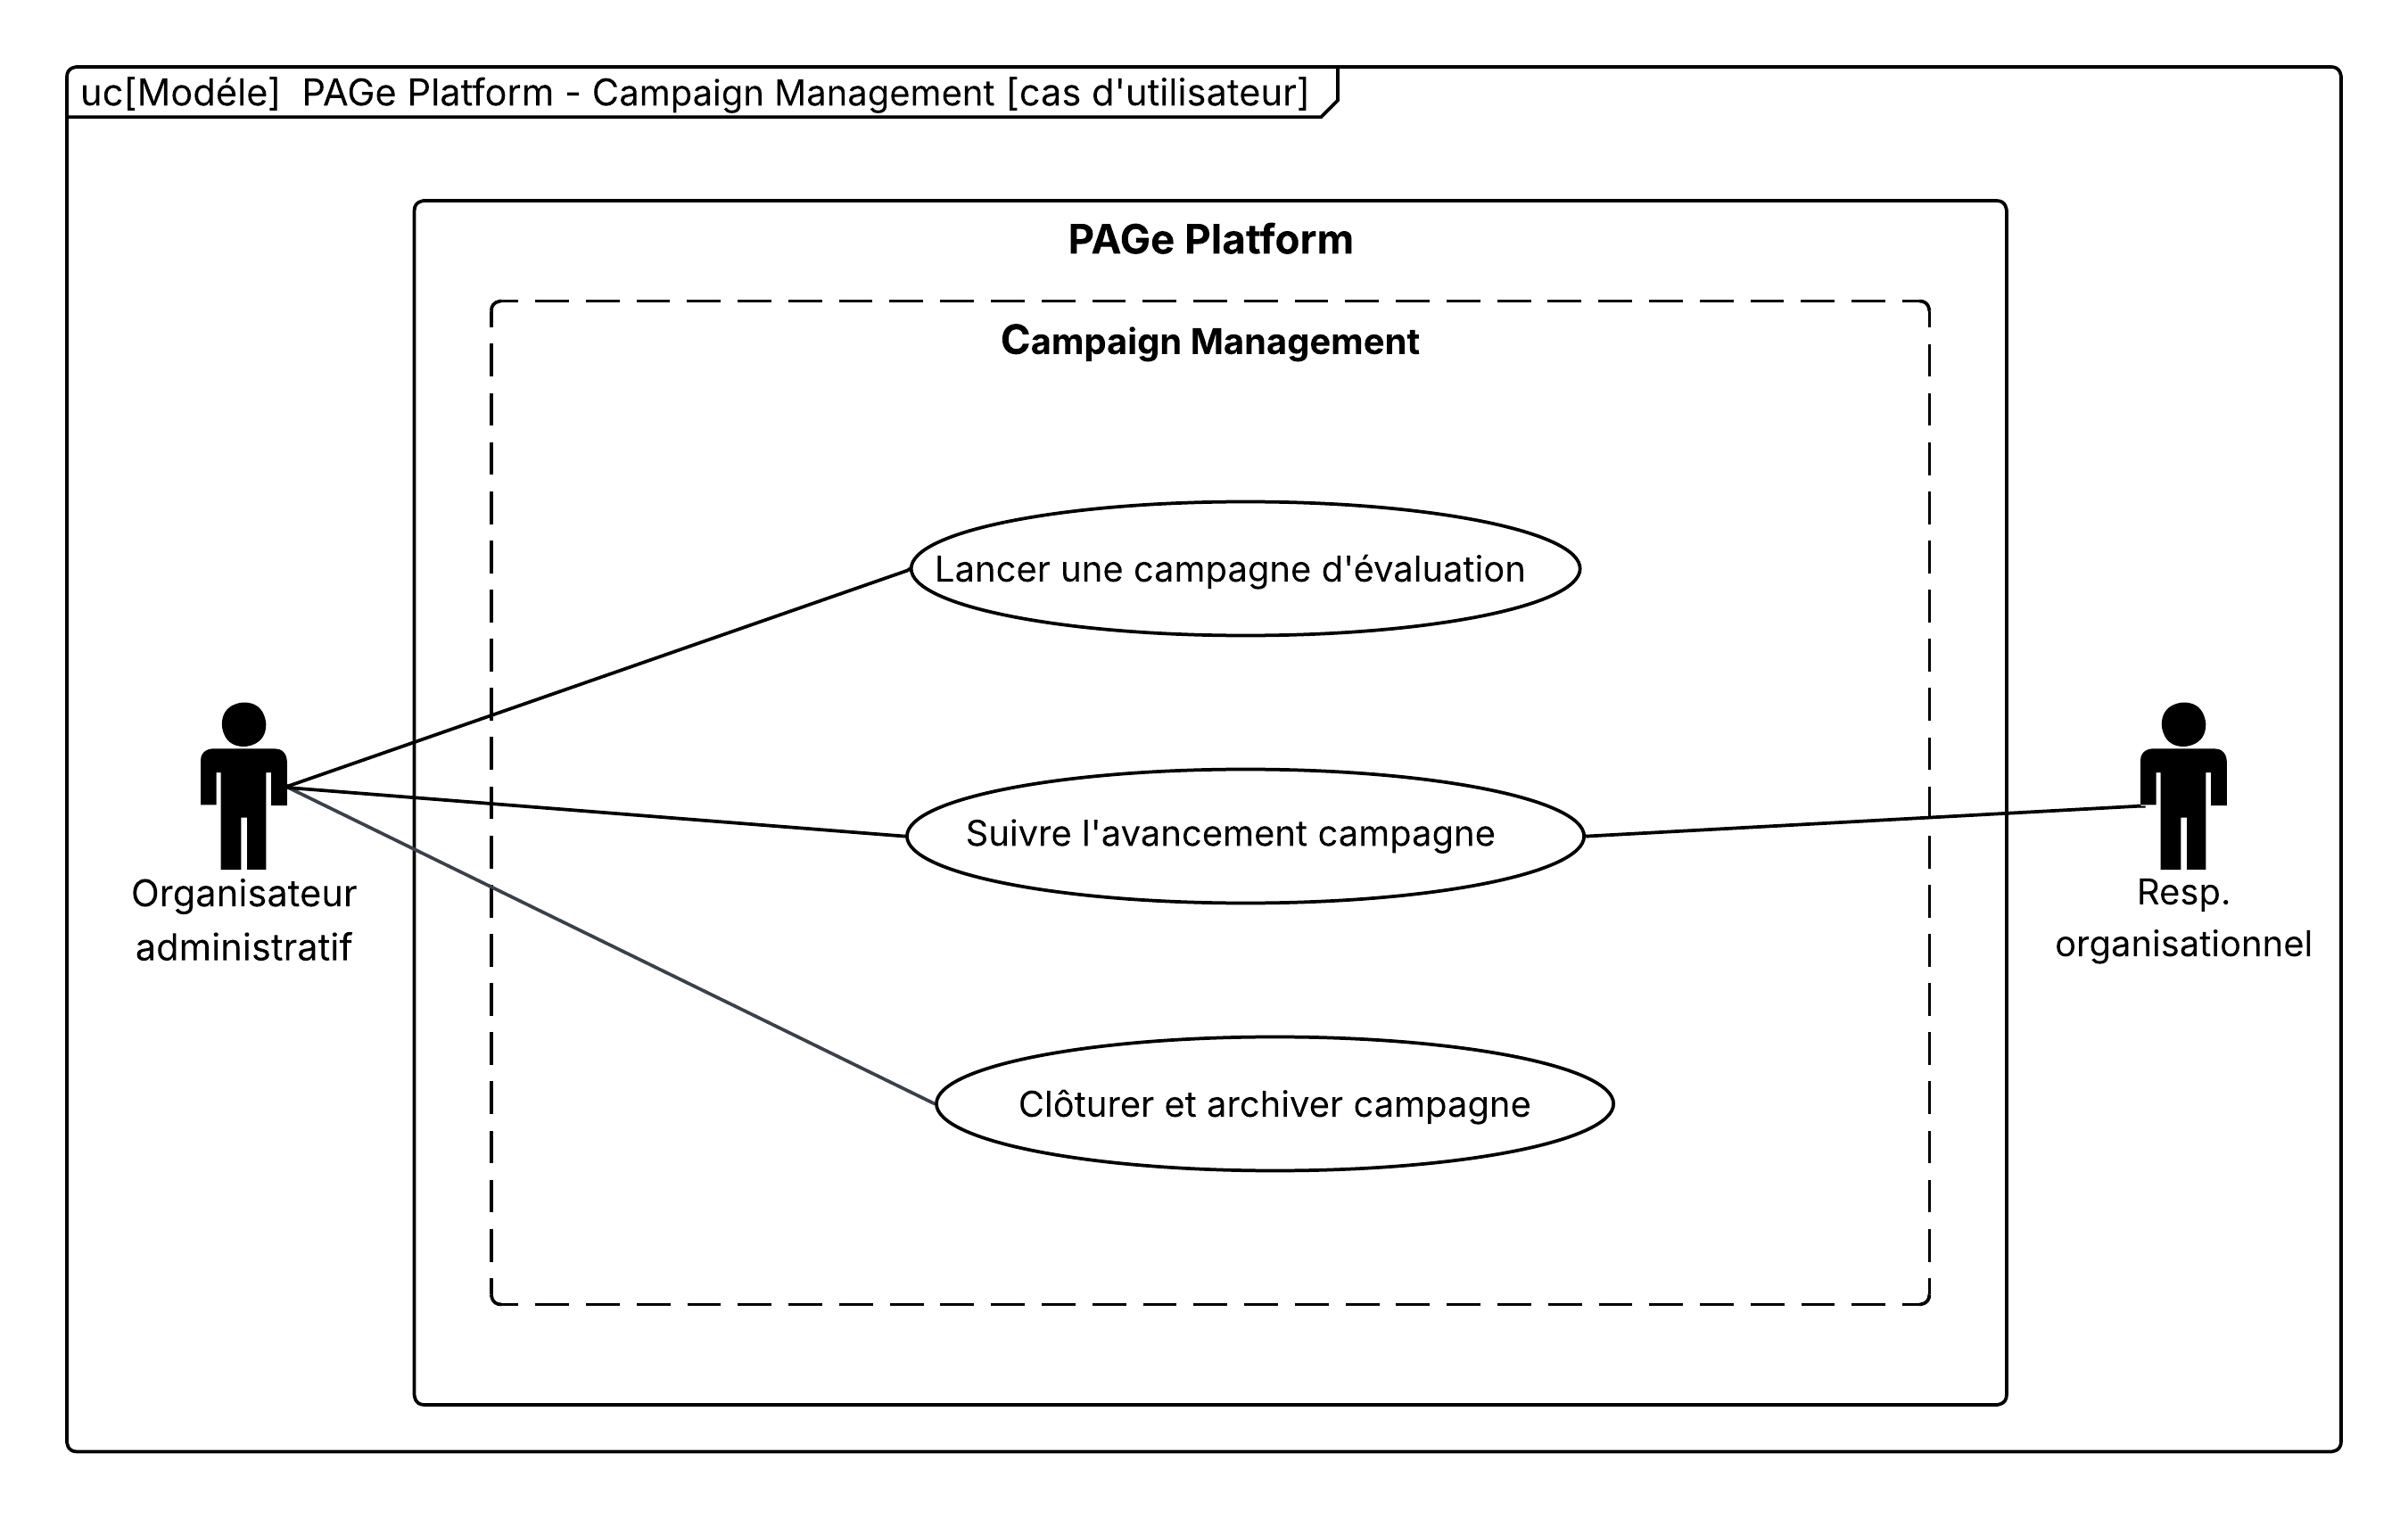
\includegraphics[width=0.80\textwidth]{figures/UC_Campaigns.png}
\caption{Diagramme de cas d'utilisation -- Gestion des campagnes}
\end{figure}

\vspace{0.5cm}

oindent\textbf{Cas d'utilisation : Lancer une campagne d'évaluation}

\begin{table}[h!]
\centering
\renewcommand{\arraystretch}{1.3}
\begin{tabular}{@{}p{0.25\textwidth}p{0.67\textwidth}@{}}
\hline
\multicolumn{2}{c}{\textbf{Sommaire d'identification}} \\
\hline
\textbf{Titre} & Lancer une campagne d'évaluation \\
\textbf{Objectif} & Créer et démarrer une nouvelle campagne pour évaluer la maturité de l'organisation. \\
\textbf{Acteurs} & Organisateur administratif \\
\hline
\multicolumn{2}{c}{\textbf{Description des scénarios}} \\
\hline
\textbf{Pré-conditions} & Le référentiel (piliers, dimensions, facteurs, items) est configuré. \\
\textbf{Scénario nominal} & L'organisateur crée une campagne en lui donnant un nom, puis la lance. Les responsables organisationnels peuvent alors y répondre. \\
\textbf{Scénarios secondaires} & Clôturer la campagne ; suivre l'avancement. \\
\hline
\end{tabular}
\caption{Description du cas d'utilisation « Lancer une campagne »}
\end{table}

% ---------- Module I-PAGe ----------
\subsection{Module I-PAGe}

\begin{figure}[h!]
\centering
\includegraphics[width=0.85\textwidth]{figures/UC_IPAGe.png}
\caption{Diagramme de cas d'utilisation -- Module I-PAGe}
\end{figure}

\vspace{0.5cm}

oindent\textbf{Cas d'utilisation : Simuler l'effet des mécanismes}

\begin{table}[h!]
\centering
\renewcommand{\arraystretch}{1.3}
\begin{tabular}{@{}p{0.25\textwidth}p{0.67\textwidth}@{}}
\hline
\multicolumn{2}{c}{\textbf{Sommaire d'identification}} \\
\hline
\textbf{Titre} & Simuler l'effet des mécanismes \\
\textbf{Objectif} & Simuler l'impact du déploiement des RMM sur les indicateurs de risque et comparer le Risk Score avant/après. \\
\textbf{Acteurs} & Organisateur administratif, Responsable organisationnel, Décideur \\
\hline
\multicolumn{2}{c}{\textbf{Description des scénarios}} \\
\hline
\textbf{Pré-conditions} & La matrice d'impact est configurée ; les niveaux de déploiement sont saisis. \\
\textbf{Scénario nominal} & L'utilisateur sélectionne un scénario de simulation, active des mécanismes avec un niveau de déploiement, et lance la simulation. Le système recalcule les indicateurs à t+1 et affiche le nouveau Risk Score. \\
\textbf{Scénarios secondaires} & Comparer plusieurs scénarios ; exporter les résultats. \\
\hline
\end{tabular}
\caption{Description du cas d'utilisation « Simuler l'effet des mécanismes »}
\end{table}

% ---------- Analytics & Reporting ----------
\subsection{Analytics et Reporting}

\begin{figure}[h!]
\centering
\includegraphics[width=0.85\textwidth]{figures/UC_Analytics.png}
\caption{Diagramme de cas d'utilisation -- Analytics et Reporting}
\end{figure}

\vspace{0.5cm}

oindent\textbf{Cas d'utilisation : Exporter les rapports}

\begin{table}[h!]
\centering
\renewcommand{\arraystretch}{1.3}
\begin{tabular}{@{}p{0.25\textwidth}p{0.67\textwidth}@{}}
\hline
\multicolumn{2}{c}{\textbf{Sommaire d'identification}} \\
\hline
\textbf{Titre} & Exporter les rapports \\
\textbf{Objectif} & Générer et télécharger un rapport PDF ou Excel contenant les résultats d'évaluation. \\
\textbf{Acteurs} & Responsable organisationnel, Décideur, Auditeur \\
\hline
\multicolumn{2}{c}{\textbf{Description des scénarios}} \\
\hline
\textbf{Pré-conditions} & Des résultats de campagne existent. \\
\textbf{Scénario nominal} & L'utilisateur sélectionne le type d'export (PDF ou Excel) et lance la génération. Le fichier est téléchargé automatiquement. \\
\textbf{Scénarios secondaires} & Choisir les données à inclure ; exporter un comparatif avant/après. \\
\hline
\end{tabular}
\caption{Description du cas d'utilisation « Exporter les rapports »}
\end{table}

% ================================================================
\section{Diagramme de classes}
Le diagramme de classes présente les entités principales du système, organisées par module. Il reflète la structure réelle du code.

\begin{figure}[h!]
\centering
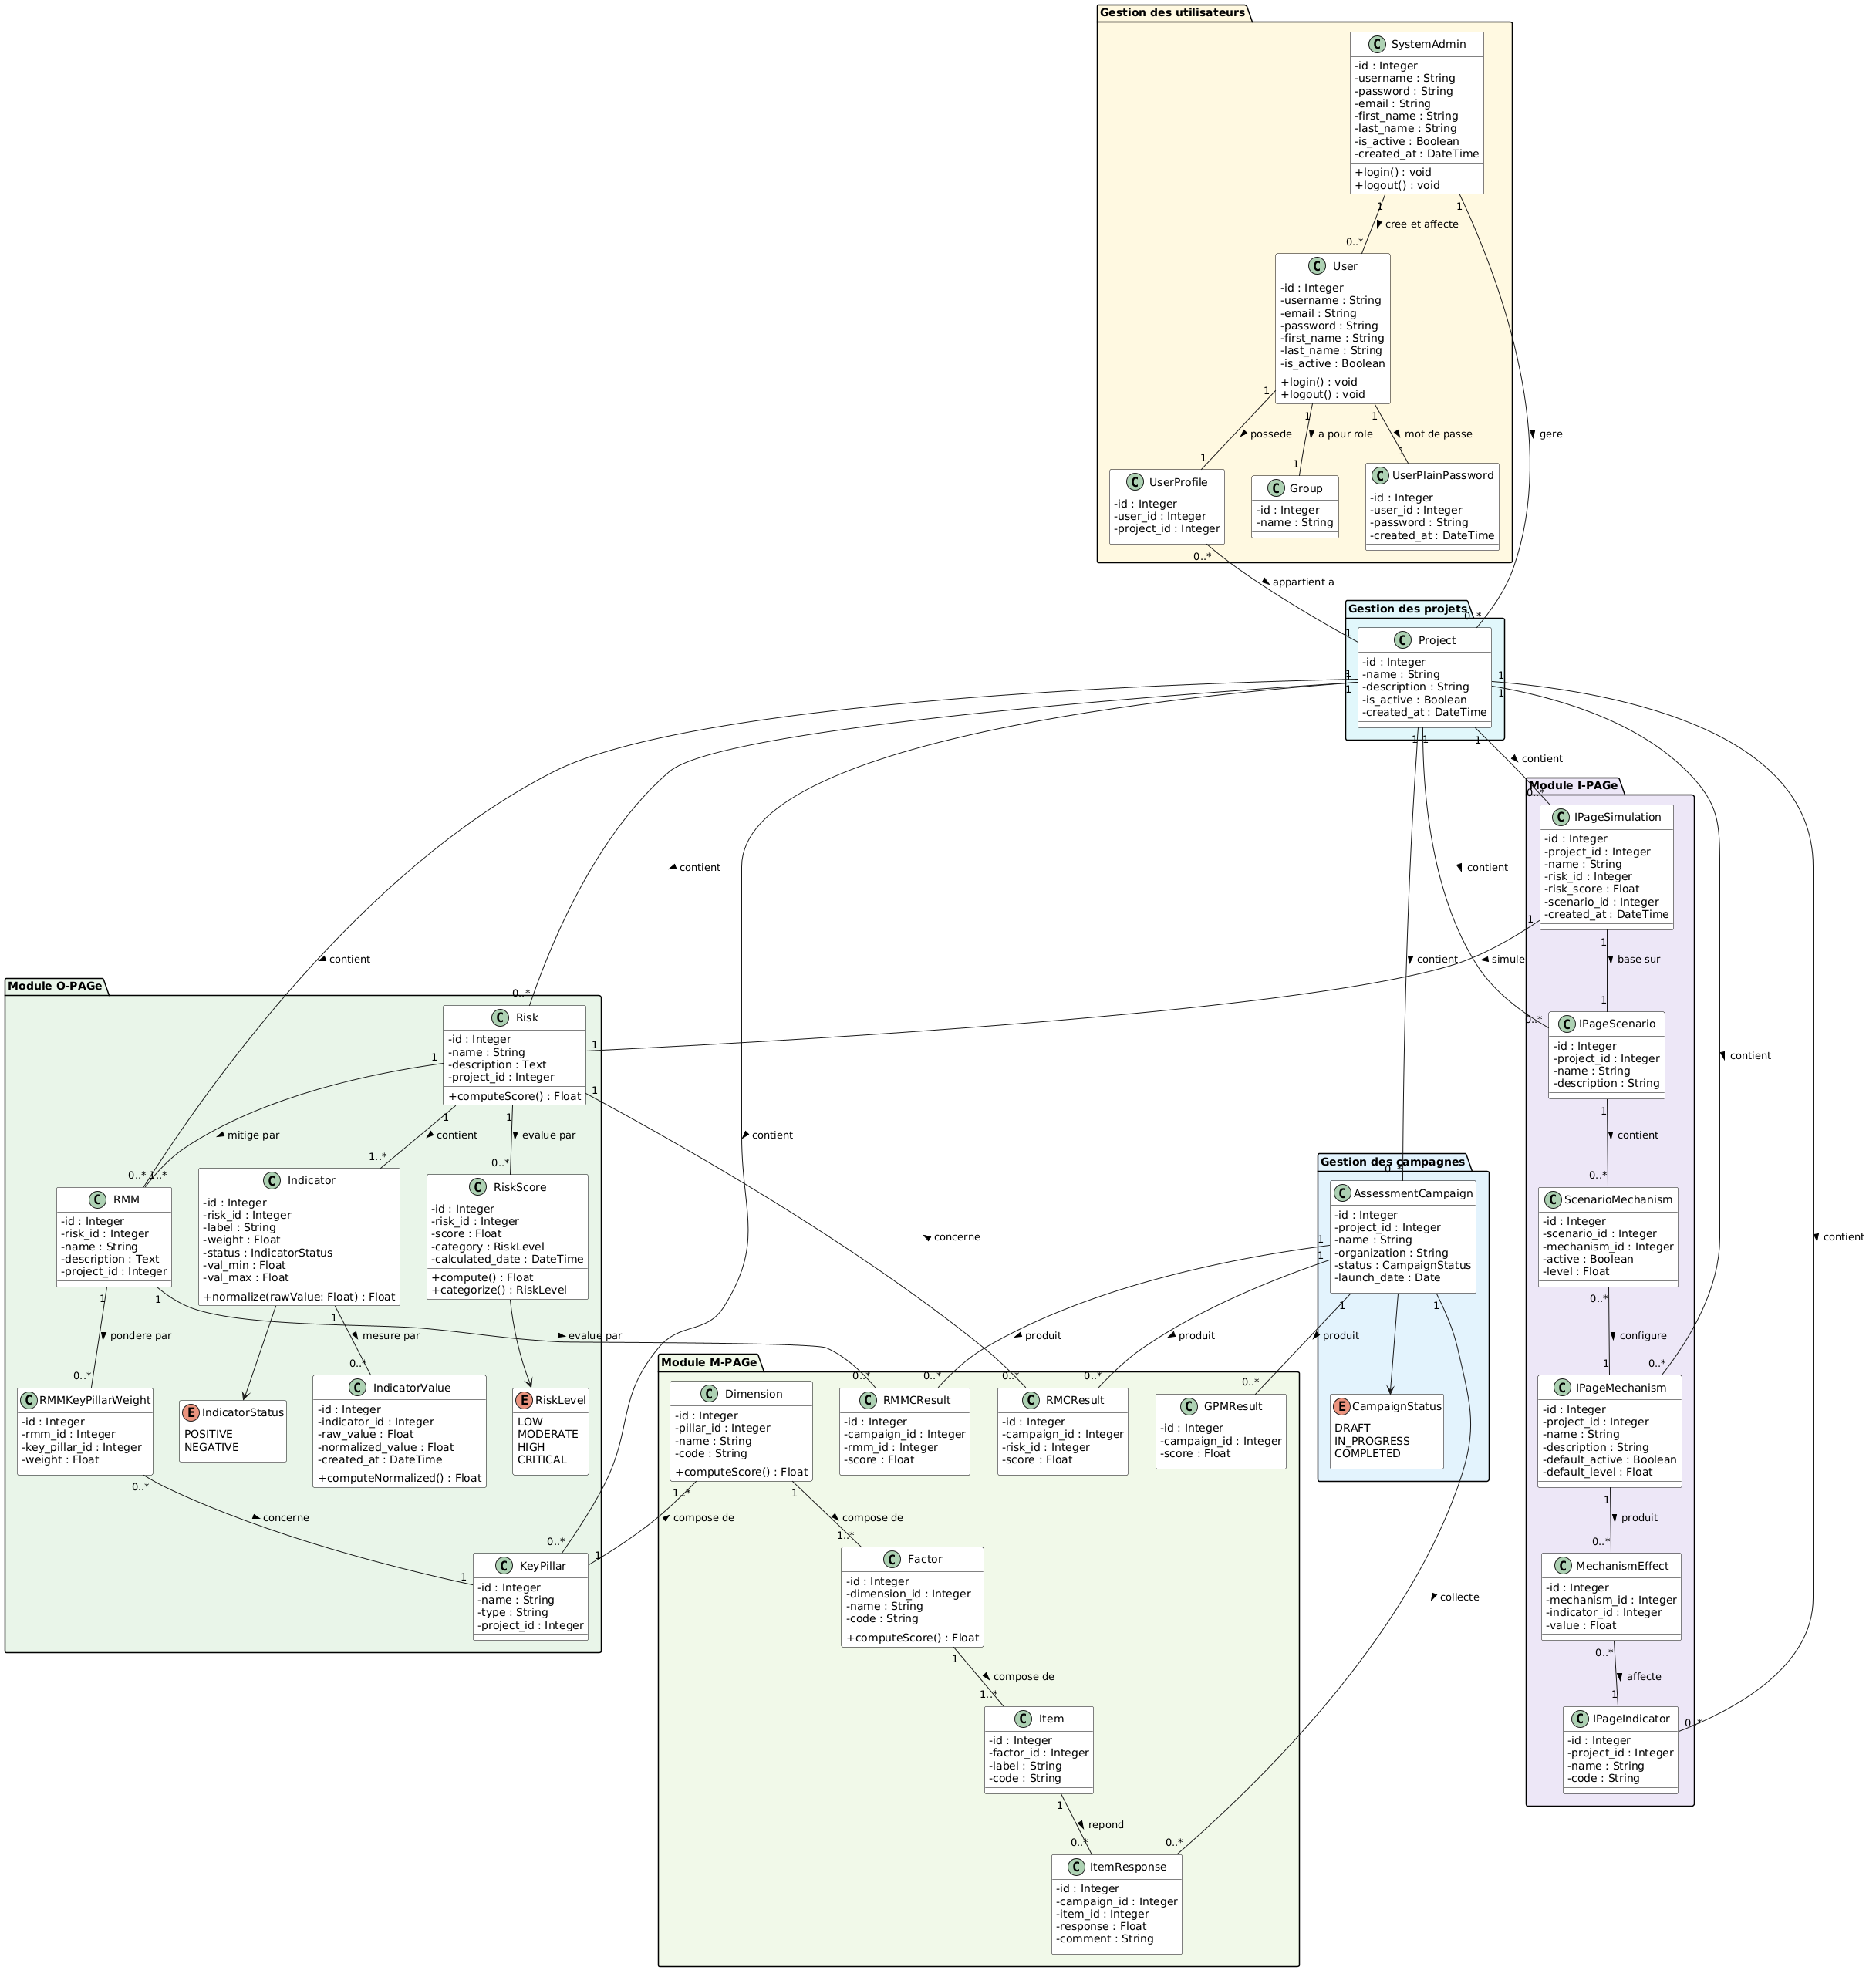
\includegraphics[width=\textwidth]{figures/class_diagram.png}
\caption{Diagramme de classes de la PAGe Platform}
\end{figure}

Les classes sont regroupées en cinq packages :
\begin{itemize}
    \item \textbf{Gestion des utilisateurs} : User, Role
    \item \textbf{Module O-PAGe} : Risk, Indicator, IndicatorValue, RiskScore
    \item \textbf{Module M-PAGe} : RMM, RMMKPWeight, KeyPillar, Dimension, Factor, Item, ItemResponse, RMMCResult, RMCResult, GPMResult
    \item \textbf{Module I-PAGe} : IPageIndicator, IPageMechanism, MechanismEffect, IPageScenario, ScenarioMechanism, IPageSimulation
    \item \textbf{Gestion des campagnes} : AssessmentCampaign
\end{itemize}

% ================================================================
\section{Modèle Conceptuel de Données (MCD)}
Le MCD représente les entités métier et leurs associations. Il a servi de base pour la conception de la base de données PostgreSQL.

\begin{figure}[h!]
\centering
\includegraphics[width=\textwidth]{figures/MCD.png}
\caption{Modèle Conceptuel de Données (MCD)}
\end{figure}

Les principales entités et leurs relations :
\begin{itemize}
    \item Un \textbf{User} possède un \textbf{Role} et gère des \textbf{Campaigns}.
    \item Un \textbf{Risk} contient plusieurs \textbf{Indicators}, est évalué par des \textbf{Risk Scores}, et est mitigé par des \textbf{RMM}.
    \item Un \textbf{Indicator} est mesuré par des \textbf{Indicator Values}.
    \item Un \textbf{RMM} dépend de plusieurs \textbf{Key Pillars} via des poids (\textbf{RMM\_KP\_Weights}).
    \item Un \textbf{Key Pillar} est composé de \textbf{Dimensions}, elles-mêmes composées de \textbf{Factors}, eux-mêmes composés d'\textbf{Items}.
    \item Les \textbf{Items} reçoivent des \textbf{Item Responses} dans le cadre d'une campagne.
    \item La \textbf{Impact Matrix} relie les RMM aux Indicators avec des coefficients d'impact.
    \item Les résultats de calcul sont stockés dans \textbf{RMMC\_Results}, \textbf{RMC\_Results} et \textbf{GPM\_Results}.
\end{itemize}

% ================================================================
\section{Architecture technique}
La plateforme suit une architecture à trois couches, déployée via Docker Compose :

\begin{figure}[h!]
\centering
\fbox{\begin{minipage}{0.88\textwidth}\centering\vspace{2.5cm}\textit{[Schéma d'architecture technique -- à insérer]}\vspace{2.5cm}\end{minipage}}
\caption{Architecture technique de la PAGe Platform}
\end{figure}

\begin{itemize}
    \item \textbf{Couche présentation} : application React/TypeScript servie par Vite, communique avec les backends via des appels API REST.
    \item \textbf{Couche métier} : deux backends Django (O-PAGe sur le port 8000, M-PAGe sur le port 8001), chacun exposant des endpoints REST via Django REST Framework. Le backend M-PAGe proxie les appels vers O-PAGe quand nécessaire.
    \item \textbf{Couche données} : une base PostgreSQL partagée entre les deux backends, administrée via pgAdmin.
    \item \textbf{Orchestration} : Docker Compose lance l'ensemble (5 conteneurs : db, opage-backend, mpage-backend, mpage-frontend, pgadmin).
\end{itemize}

% ================================================================
\section{Conclusion}
Ce chapitre a présenté l'analyse des besoins à travers les diagrammes de cas d'utilisation et la description des scénarios pour chaque module. Nous avons aussi présenté le diagramme de classes, le MCD et l'architecture technique de la plateforme. Le chapitre suivant détaille la réalisation concrète de l'application.
